\section{Introduction}
This chapter outlines the methodology for the multiple knapsack assignment problem approach utilized in this research. Described in depth are the fuel estimation equations and the distance formula used in the model. Then the mathematical model is outlined. Lastly detailed are how the model inputs are prepared and the solution is processed.

\section{Fuel Estimation} \label{sec_fuelEquations}
In \cite{Reiman2014} Reiman developed fuel regression equations based on flight data from aircraft performance manuals for the C-17, C-5, and C-130.  These equations model the fuel, in kilo-pounds, required of the three aircraft types to climb, cruise and descend based on the aircraft gross weight, altitude and distance to travel.  While the equations allow for a user-defined altitude, the analysis was based on using the optimal cruise altitude for an aircraft's maximum gross takeoff weight. These aircraft assumptions are listed in Table \ref{tableAssume}.  
\begin{table}[h!]
\centering
\caption{Aircraft Specific Payload Movement Assumptions \cite{Reiman2014}}
\label{tableAssume}
\begin{tabular}{@{}lccc@{}}
\toprule
 & C-5 & C-17 & C-130 \\ \midrule
Operating Weight $\omega_{op}$ & 380 & 282.5 & 78 \\
Max Gross Takeoff Weight $\omega_{mgt}$ & 769 & 585 & 155 \\
Fuel Capacity $\omega_{fcap}$ & 347 & 241.36 & 62 \\
Aircraft Max Payload, $\omega_{apmax}$ & 270 & 170.9 & 53 \\
Reserve Fuel $\omega_{frc}$& 23.45 & 21.44 & 4 \\
Alternate Fuel \} $\omega_{fah}$ & 23.45 & 21.44 & 4 \\
Holding Fuel  & 17.59 & 16.08 & 0 \\
Start Taxi Takeoff Fuel $\omega_{fstto}$ & 3 & 4.5 & 0.67 \\
Approach $\omega_{fapp}$ & 7 & 2.67 & 0.7 \\ \bottomrule
\end{tabular}
\end{table}


Values for each regression model depend on the weights from Table \ref{tableAssume} as well as calculated values from one or both of the other regression models.  The combination of given weights from Table \ref{tableAssume} and the calculated weights result in Equation \ref{eq_fuel_ramp} for the ramp fuel weight. Equation  \ref{eq_fuel_ramp} plays a part in Equation \ref{eq_fuel_climb}, the model calculating the fuel required to climb.  The regression coefficient values for the climb equation are in Table \ref{tableClimb}. The regression coefficient values in Table \ref{tableDescent} are for Equation \ref{eq_fuel_descent}, the model calculating the fuel required to descend.  \newline
\begin{equation}
\label{eq_fuel_ramp}
\omega_{rf}=\omega_{fstto}+\omega_{fc}+\omega_{ff}+\omega_{fd}+ \omega_{fapp}+\omega_{frc}+\omega_{fah}
\end{equation}
% \begin{equation}
% \label{eq_grossweight_descent}
% \omega_{gd}= \omega_g-\omega_{fstto}-\omega_{fc}-\omega_{ff}
% \end{equation}   
\begin{equation}
\label{eq_fuel_climb}
\omega_{fc}=\beta_0+\beta_1\alpha+\beta_2\alpha^2+\beta_3\alpha^3+\beta_4\omega+\beta_5\omega^2+\beta_6\omega^3+10^{-6}\beta_7\alpha^2\omega^3+10^{-6}\beta_8\alpha^2\omega^3
\end{equation}
\begin{equation}
\label{eq_fuel_descent}
\omega_{fd}=\beta_0+\beta_1\omega_{gd}+\beta_2\omega_{gd}^2+\beta_3\alpha+\beta_4\alpha\omega_{gd}
\end{equation}
\setlength{\jot}{-1ex}
\renewcommand*\arraystretch{.8}
where:
\begin{align*}
\omega_{fc} &= \text{Fuel to Climb in Klbs}\\
\omega_{fd} &= \text{Fuel to Descend in Klbs}\\
\alpha &= \text{Altitude in Thousands of Feet}\\
\omega &=\text{Aircraft Gross Weight in Klbs at Climb Start}\\
&=\omega_{rf}+\omega_{op}+\omega_p\\
\omega_{gd} &=\text{Aircraft Gross Weight in Klbs at Descent Start}\\
&= \omega-\omega_{fstto}-\omega_{fc}-\omega_{ff}\\
\omega_{fstto} &= \text{Fuel for Start, Taxi, and Takeoff in Klbs}\\
\omega_{ff} &=\text{Fuel to Cruise in Klbs}
\end{align*}
%
\begin{table}[h!]
\begin{minipage}{.5\linewidth}
\centering
\caption{Climb $\omega_{fc}$ Regression Terms \cite{Reiman2014}}
\label{tableClimb}
\begin{tabular}{@{}lccc@{}}
\hline
\hline
& C-5  & C-17 & C-130\\\hline
$\beta_0$ & -3.0115 & -4.7054 & -1.067 \\
$\beta_1$ & 0.3192 & 0.2869 & 0.0669 \\
$\beta_2$ & -0.0082 & -0.007 & -0.0022 \\
$\beta_3$ & 9.50E-05 & 7.10E-05 & 3.00E-05 \\
$\beta_4$ & 0.0164 & 0.0267 & 0.0218 \\
$\beta_5$ & -3.30E-05 & -5.90E-05 & -0.0002 \\
$\beta_6$ & 2.20E-08 & 4.80E-08 & 5.20E-07 \\
$\beta_7$ & 3.70E-05 & 6.70E-05 & 0.0003 \\
$\beta_8$ & 7.10E-08 & -2.10E-07 & 1.30E-05\\ \hline
\end{tabular}
\end{minipage}
\begin{minipage}{.5\linewidth}
\centering
\caption{Descent $\omega_{fd}$ Regression Terms \cite{Reiman2014}}
\label{tableDescent}
\begin{tabular}{@{}lccc@{}}
\hline
\hline
& C-5  & C-17 & C-130\\\hline
$\beta_0$ & -1.9673 & 0.2574 & -0.0513 \\
$\beta_1$ & 0.0128 & 0.0005 & -0.0012 \\
$\beta_2$ & 1.34E-05 & -8.50E-07 & 1.38E-05 \\
$\beta_3$ & 0.1254 & 0.0108 & 0.0367 \\
$\beta_4$ & 0.0004 & 3.20E-05 & -0.0002\\\hline
\end{tabular}
\end{minipage}
\end{table}

\pagebreak The regression coefficient values for Equation \ref{eq_fuel_cruise}, the model calculating the fuel required to cruise, are in Table \ref{tableCruise}. While the weight of the reserve fuel and the alternate fuel are not planned to be consumed, they are a necessary part in the fuel equations because they add to the overall ramp fuel weight and weight of the plane over the course of the flight.

\setlength{\jot}{+1ex}
\begin{equation}
\label{eq_fuel_cruise}
\begin{aligned}
\omega_{ff}=&-\frac{B}{3A}-\frac{1}{3A} \sqrt[3]{\frac{1}{2}[2B^3-9ABC+27A^2D+\sqrt[]{(2B^3-9ABC+27A^2D)^2-4(B^2-3AC)^3]}}\\
&-\frac{1}{3A}\sqrt[3]{\frac{1}{2}[2B^3-9ABC+27A^2D-\sqrt[]{(2B^3-9ABC+27A^2D)^2-4(b^2-3AC)^3}]}
\end{aligned}
\end{equation}


\setlength{\jot}{-1ex}
 where (all weights in Klbs):\\
 $A =\frac{\beta_4}{3}\\$
 $B =(\frac{\beta_3}{2}+\beta_4(\omega_{op}+\omega_{frc}+\omega_{fah}+\omega_p)+\frac{\beta_5}{2}\alpha)$\\
 $C=\beta_0+\beta_1\alpha+\beta_2\alpha^2+\beta_3(\omega_{op}+\omega_{frc}+\omega_{fah}+\omega_p)+$\\
 \text{\hspace{9mm}}$\beta_4(\omega_{op}+\omega_{frc}+\omega_{fah}+\omega_p)^2+\beta_5\alpha(\omega_{op}+\omega_{frc}+\omega_{fah}+\omega_p)$\\
 $D= -\delta$\\
 $\delta = \text{Distance in NMs}$\\
% $\omega = \text{Aircraft Gross Weight}$\\
 %\text{\hspace{5mm}}$=\omega_{op}+\omega_{frc}+\omega_{fah}+\omega_p+f$\\
 $\omega_{op} = \text{Operating Weight}$\\
 $\omega_{frc}=\text{Reserve/Contingency Fuel Weight}$\\
 $\omega_{fah}=\text{Alternate/Holding Fuel Weight}$\\
 $\omega_p= \text{Payload Weight}$\\
 %$f= \text{Fuel Consumed}$\\
 $\omega_{ff}= \text{Fuel to Cruise in Klbs}$\\
 \setlength{\jot}{+1ex}


\begin{table}[h!]
\centering
\caption{Cruise $\omega_{ff}$ Regression Terms \cite{Reiman2014}}
\label{tableCruise}
\begin{tabular}{@{}lccc@{}}
\hline
\hline
 & C-5 & C-17 & C-130 \\ \hline
$\beta_0$ & 24.538 & 31.735 & 58.829 \\
$\beta_1$ & 0.5511 & 0.9897 & 3.5292 \\
$\beta_2$ & 0.0002 & -0.0043 & -0.0098 \\
$\beta_3$ & -0.0318 & -0.0642 & -0.2384 \\
$\beta_4$ & 0.000019 & 0.000058 & 0.001 \\
$\beta_5$ & -0.0005 & -0.0011 & -0.0155
\end{tabular}
\end{table}

\section{Distance Estimation}
The solution to this application of the MKAP relies heavily on Reiman's \cite{Reiman2014} fuel estimation equations. One factor in these equations is distance. Utilized in both Reiman's work and in this research is the Vincenty distance formula \cite{Vincenty1975DirectEquations}. Instead of assuming a straight line distance and using the Pythagorean Theorem, or assuming a spherical Earth and using the great-circle distance, the Vincenty Inverse Method assumes the Earth is a flattened spheroid and iteratively calculates distance via ellipsoidal geometry given the latitude and longitude of both the source and the destination points.  The reference used for Earth's geospatial properties in Reiman's and this work is the World Geodetic System 1984 (WGS84) \cite{WGS}.\par
The maximum distance an aircraft can traverse is estimated assuming that cruise and descent fuel have little impact on distance. Equation \ref{eq_fuel_cruise} is used, setting the fuel consumed equal to the maximum amount of fuel an aircraft is allowed to carry given a payload weight, Equation \ref{eq_maxFuel}, and solving for distance.
\begin{equation}
\label{eq_maxFuel}
maxFuel=min(\omega-\omega_{op}-\omega_p, \hspace{3mm} \omega_{fcap}) 
\end{equation}
\newpage
\section{Mathematical Model} \label{sec_mathModel}
The mathematical program for the problem uses the fuel equations in not only the constraints, but also the objective function, Equation \ref{eq_obj}.  There are two sets of bases, one acting as a supplier and one as the demand. Expected demand is used as the constraint in Equation \ref{eq_demand} for the amount required to be sent to the demanding base from all suppliers. The aircraft is a largely constraining factor in the problem. Each aircraft has a maximum weight for payload, takeoff, and fuel, shown in Table \ref{tableAssume} and accounted for in Equations \ref{eq_payloadCap}, \ref{eq_maxGrosstakeoff}, \ref{eq_fuelCap}, respectfully. Aircraft also have a given amount of floor space for cargo \cite{C5}\cite{c-17}\cite{c130}, therefore the amount of cargo cannot exceed the given floor space in Equation \ref{eq_spaceCap}. Cargo is assumed to be on standard pallets, and is constrained to the properties associated with a standard pallet of item type $K$ in Equation \ref{eq_IntegerPAllets}; there are no partial pallets. A supplying base has a limit on the number of a specific item type $K$, and is only allowed to send what is available in inventory in Equation \ref{eq_supplyconstraint}. Equations \ref{eq_AC_Assignment} and \ref{eq_binaryAssignment} are the assignment equations, ensuring an aircraft is only allowed to fly the cargo between one supply-demand pairing.\\  

\textbf{Sets:}\newline
$I$  set of supply bases, indexed by $i$\\
$J$  set of demand bases, indexed by $j$\\
$K$  set of item types, indexed by $k$\\
$L$  set of aircraft, indexed by $l$\newline

\textbf{Decision Variables:}  \newline
$x_{ij}^{kl}$  number of pallets of item $k$ to fly on aircraft $l$ from base $i$ to base $j$.  \newline
$y_{ij}^l$  assignment of aircraft $l$ to deliver from base $i$ to base $j$.  \newline

\textbf{Parameters:} \newline  
$D_j^{k}$  expected demand of base $j$ for item $k$   \newline 
$supply_i^k$  supply inventory of item $k$ at base $i$   \newline 
$w_{k}$  weight of item type $k$  \newline 
$\omega_{mgt}^{l}$ maximum gross takeoff weight for aircraft $l$   \newline
$\omega_{apmax}^l$ maximum payload weight for aircraft $l$ \newline
$\omega_{fcap}^l$ maximum fuel weight for aircraft $l$ \newline
$\omega_{rf}^l$ ramp fuel weight for aircraft $l$ \newline
$\omega_{frc}^l$ reserve/contingency fuel weight for aircraft $l$ \newline
$\omega_{fah}^l$ alternate/holding fuel weight for aircraft $l$ \newline
$f_{ij}^l$ total fuel consumed in Klbs, $f=\omega_{rf}-\omega_{frc}-\omega_{fah}$ \newline
$space^{l}$  space capacity of cargo floorspace of aircraft type $l$   \newline 
$fuelPrice$ current market price of fuel per Klb\\ 
\newpage
\textbf{Objective Function:}  
\begin{equation}
\label{eq_obj}
\min \hspace{5mm}
fuelPrice*\sum_{i\in I}\sum_{j\in J}\sum_{l\in L}(f_{ij}^l|y_{ij}^l \text{ and } x_{ij}^{kl}) 
%(\omega_{fstto}^{l}+\omega_{fc}^{ijl}+\omega_{ff}^{ijl} + \omega_{fd}^{ijl}+\omega_{app}^{l})
\end{equation}

\textbf{Subject to:}
\begin{align}
\sum_{i\in I}\sum_{l\in L}x_{ij}^{kl}&= D_j^{k} &\forall \hspace{2mm} j \in J \text{, } k\in K \label{eq_demand}\\
\sum_{k\in K}w_{k}x_{ij}^{kl}&\leq \omega_{apmax}^{l}y_{ij}^l &\forall \hspace{2mm} i \in I \text{, } j\in J \text{, } l \in L \label{eq_payloadCap}\\
\omega_{g}^{ijl}&\leq \omega_{mgt}^l &\forall \hspace{2mm} i \in I \text{, } j\in J \text{, } l \in L \label{eq_maxGrosstakeoff}\\
\omega_{rf}^{ijl} &\leq \omega_{fcap}^l &\forall \hspace{2mm} i \in I \text{, } j\in J \text{, } l \in L \label{eq_fuelCap}\\
\sum_{k\in K}x_{ij}^{kl} &\leq space^{l}y_{ij}^l  &\forall \hspace{2mm}  i\in I \text{, } k\in K \text{, } l\in L \label{eq_spaceCap}\\
\sum_{j\in J}\sum_{l \in L}x_{ij}^{kl} &\leq supply_i^k &\forall\hspace{2mm} i \in I \text{, } j\in J \label{eq_supplyconstraint}\\
x_{ij}^{kl}& \text{  integer}  \hspace{15mm}&\forall \hspace{2mm} i\in I \text{, } j \in J \text{, } k\in K \text{, } l \in L \label{eq_IntegerPAllets}\\ 
\sum_{i \in I}\sum_{j\in J}y_{ij}^l &\leq 1 &\forall \hspace{2mm} l \in L \label{eq_AC_Assignment}\\
y_{ij}^l &\in \{0,1\} &\forall \hspace{2mm} i \in I \text{, } j \in J \text{, } l\in L \label{eq_binaryAssignment}
\end{align}

\pagebreak
\section{Assumptions} \label{sec_assumptions}
Several assumptions were made in the interest of simplifying the computational complexity of the model.  While there are many bases which can act as supply and demand bases, the pavement of supply and demand locations sampled for this problem can handle the take-off and landing of any of the three types of aircraft with their respective maximum payloads.  Aircraft
maximum payload weight, maximum gross takeoff weight and operating weight are assumed to
be fixed as shown in Table \ref{tableAssume}.\par
It is assumed airfields are available for routing of aircraft, however, enroute stops are not calculated based on actual base locations, but are equidistant points on the direct route between supply demand pairings.  The necessity of one or more enroute stops for a given mission design series (MDS) and payload is calculated in Algorithm \ref{alg_numStops}. The number of stops is determined by dividing the Vincenty distance \cite{Vincenty1975DirectEquations} by the calculated maximum distance the aircraft can fly carrying the payload and rounding this number down to the closest integer. For example, if the distance between the pairings is less than the maximum distance at maximum payload weight, then the ratio would be less than one. This rounds down to a necessity of zero enroute stops.  No cargo is delivered or exchanged at enroute stops, however fuel tanks are re-filled to maximum capacity.\par
\begin{algorithm}[H]
\caption{Number of Stops}
\label{alg_numStops}
\begin{algorithmic}
\Function {numStops}{MDS, distance, payload}
		\State $numberStops =$ numStops(selectMDS, distance, payload)
        \State $stopDist =$ maxDistance(payload)
    	\State $numStops = roundDown(distance / stopDist)$
\EndFunction
\end{algorithmic}
\end{algorithm}
Demand bases do not have inventory restriction and have the equipment necessary to receive and handle any items. Weather is not a limiting factor and is not taken into account for routing or fuel cost. Reserve, contingency, alternate and holding fuels are safety fuels that are carried but not consumed.  The model assumes that aircraft are prepositioned to fulfill assignment pairings, and need not fly from another location to get to the supply base. The cost of prepositioning aircraft at supply locations is not a factor. Time is also not a factor.  There are adequate crew to fulfill the flight requirements of assignments. 

\section{Math Model Modifications} \label{sec_mathModelMod}
Complications implementing the fuel calculations within the General Algebraic Modeling System (GAMS) resulted in a modification to the mathematical model in the GAMS program. The objective function that drives the solution in GAMS was altered to solve minimizing an approximation to the fuel cost. Prior to running the GAMs model, the fuel cost of a specific aircraft flying from one supply location to one demand location is calculated for the plane carrying the maximum payload as well as the base fuel cost for flying no payload, Equation \ref{eq_baseFuelCost}. The cost per payload kilopound is calculated in Equation \ref{eq_costPerPayload} by taking the difference between these two values and dividing it by the maximum payload weight for the specific aircraft.
\begin{equation}
\label{eq_baseFuelCost}
baseFuelCost_{ij}^l=f_{ij}^l(zeroPayload)
\end{equation}
\begin{equation}
\label{eq_costPerPayload}
fuelCost_{ij}^l=\frac{f_{ij}^l(maxPayload)-baseFuelCost_{ij}^l}{\omega_{apmax}^l}
\end{equation}

Multiplying the payload by the cost per payload and adding it to the cost of flying the aircraft while empty results in the approximated cost of carrying the payload that is used in the GAMS objective function, Equation \ref{eq_obj2}. By altering the objective function from Equation \ref{eq_obj} to Equation \ref{eq_obj2}, the GAMS model no longer requires constraint Equations \ref{eq_maxGrosstakeoff} or \ref{eq_fuelCap}. Finally, to focus on the aspect of demand in the analysis, supply is assumed to be unlimitied, therefore the supply constraint, Equation \ref{eq_supplyconstraint}, is also removed.
\begin{equation}
\label{eq_obj2}
\min \hspace{5mm}
fuelPrice*\sum_{i\in I}\sum_{j\in J}\sum_{k\in K}\sum_{l\in L}(w_{k}x_{ij}^{kl}*fuelCost_{ij}^{l}+baseFuelCost_{ij}^l)
\end{equation}
\textbf{Subject to:}
\begin{align*}
\sum_{i\in I}\sum_{l\in L}x_{ij}^{kl}&= D_j^{k} &\forall \hspace{2mm} j \in J \text{, } k\in K \tag{\ref{eq_demand}}\\
\sum_{k\in K}w_{k}x_{ij}^{kl}&\leq \omega_{apmax}^{l}y_{ij}^l &\forall \hspace{2mm} i \in I \text{, } j\in J \text{, } l \in L \tag{\ref{eq_payloadCap}}\\
\sum_{k\in K}x_{ij}^{kl} &\leq space^{l}y_{ij}^l  &\forall \hspace{2mm}  i\in I \text{, } k\in K \text{, } l\in L \tag{\ref{eq_spaceCap}}\\
x_{ij}^{kl}& \text{  integer}  \hspace{15mm}&\forall \hspace{2mm} i\in I \text{, } j \in J \text{, } k\in K \text{, } l \in L \tag{\ref{eq_IntegerPAllets}}\\ 
\sum_{i \in I}\sum_{j\in J}y_{ij}^l &\leq 1 &\forall \hspace{2mm} l \in L \tag{\ref{eq_AC_Assignment}}\\
y_{ij}^l &\in \{0,1\} &\forall \hspace{2mm} i \in I \text{, } j \in J \text{, } l\in L \tag{\ref{eq_binaryAssignment}}
\end{align*}

\section{Solution Pre-processing} \label{sec_solutionPreProcessing}
Many of the subroutines and functions, written in Microsoft Excel Visual Basic for Applications (VBA), are used for data collection and pre-processing. Initially, the user is prompted to select the supply and demand airfields from a list of 5342 airfields from the Digital Aeronautical Flight Information File (DAFIF) database. The user may manually add the specific International Civil Aviation Organization airport code (ICAO) to the supply base list, or they may use a button to populate the list with the known channel continental United States (CONUS) supply bases, or, for completely proof of concept purposes, the user may use a button to randomly populate the list with a specific number of supply bases. With the selection of airfields the user is requested to input the inventory of the supply bases and the requirements for the demand bases of two cargo types, high priority, ``Priority 1" or ``Super/999/1," cargo and regular priority, ``Priority 2/3" cargo. They may do this manually, or may use a button on the respective pages to randomly populate the supply and demand. Up to this point, a supply sheet and a demand sheet have been created. Lastly, the user is asked to add the number of available C-5Bs, C17s, and C-130J-30s via the aircraft selection form, seen in Figure \ref{fig_acSelectionForm}. \par
\begin{figure}[H]
\centering
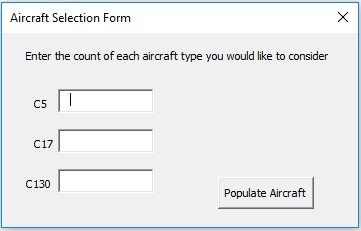
\includegraphics[width=80mm]{acSelectionForm.PNG}
\caption{Aircraft Selection Form}
\label{fig_acSelectionForm}
\end{figure}
Upon clicking the ``Populate Aircraft'' button, many subroutines and functions are called upon to create the aircraft page. This lists available aircraft, their associated parameters such as maximum takeoff weight and fuel capacity, and the calculated aircraft costs per payload and baseline fuel costs to fly between the source and destination pairings. The main subroutine called to perform this page creation is called GetDistance. As seen in Algorithm \ref{alg_getDistance}, the GetDistance subroutine initially finds the latitude and longitude for the supply base, then iterates through the demand bases. For each demand base, the latitude and longitude is found, then the program iterates through all available aircraft. The vincentyDistance function is called to calculate the Vincenty distance between the supply and demand base and fuel function is called to calculate the fuel cost given the distance, MDS, and payload.  For the base fuel calculation the payload is zero. For the max fuel calculation the payload is the maximum payload for the given aircraft type.\par
\begin{algorithm}[H]
\caption{Sub Routine GetDistance}
\label{alg_getDistance}
\begin{algorithmic}
\For{each supply base $i\in I$}
	\For{all $airfields$}
    	\If {$airfield=supply base$}
          	\State $lat1=airfield.latitude$
            \State $long1=airfield.longitude$
            \State \textbf{exit for} all airfields
        \EndIf
	\EndFor
    \For{each demand base $j\in J$}
		\For{all $airfields$}
			\If {$airfield=supply base$}
				\State $lat2=airfield.latitude$
            	\State $long2=airfield.longitude$
                \State $distance=$ vincentyDistance(lat1, long1, lat2, long2)
                \For {all aircraft $l \in L$} 
                	\State $MDS= aircraft.MDS$
                    \State $maxPayload=aircraft.maxpayload$
					\State $baseFuel=$fuel(MDS, distance, payload=0)
					\State $payloadFuel=$ fuel(MDS, distance, payload=maxpayload)
					\State $maxFuel= (payloadFuel-baseFuel)/maxPayload$
                	\State \textbf{write} supplyBase, demandBase, baseFuel, maxFuel 
                \EndFor
                \State \textbf{exit for} all airfields
        	\EndIf
      	\EndFor
	\EndFor
 \EndFor
\end{algorithmic}
\end{algorithm}
As seen in Algorithm \ref{alg_fuel}, the fuel function calls upon the numStops function to provide the number of stops the aircraft requires given payload and distance and calls upon the fuelCalculation function to calculate the amount of fuel consumed for a given aircraft type, distance, number of stops, and payload amount. The fuelCalculation function calculates fuel consumption using the fuel equations detailed in Section \ref{sec_fuelEquations}. All functions and subroutines may be found in Appendix \ref{A01_VBA}. 
\begin{algorithm}[H]
\caption{Fuel Calculations}
\label{alg_fuel}
\begin{algorithmic}
\Function {fuel}{MDS, distance, payload}
	\State $numberStops = $numStops(MDS, distance, payload)
    \State $fuel = $fuelCalculations(MDS, distance, payload, numberStops)
\EndFunction
\end{algorithmic}
\end{algorithm}

\section{Solution Processing} \label{sec_solutionProcessing}

 GAMS Data eXchange (GDX) facilities pull data and parameters from the Excel workbook into GAMS. After the pre-processing detailed in Section \ref{sec_solutionPreProcessing}, the Excel workbook provides GAMS with the sets of supply bases and demand bases with their respective associated inventory and demand, and the set of available aircraft, with their associated parameters of operating weight, fuel capacity, maximum gross takeoff weight, average altitude, maximum payload capacity, and the aircraft's baseline cost and cost per payload pound for all pairings of supply and demand bases. The modified model from Section \ref{sec_mathModelMod} is solved in GAMS for a nonlinear mixed integer program using BARON \cite{Klnc2018ExploitingBARON}. The GAMS code may be found in Appendix \ref{A02_GAMS}. Once solved, GDX writes the aircraft assignments, payload weights, cargo allocations, and demand base requirements shortage and overage to sheets in the same Excel workbook from which the data is called.  The finalCost subroutine, Algorithm \ref{alg_finalCost}, then calls upon the fuel function and uses these outputs to calculate the final total cost. 
 \begin{algorithm}
 \caption{Sub Routine finalCost}
 \label{alg_finalCost}
 \begin{algorithmic}
 \For{each Supply-Demand base combination}
    \For{each allocated aircraft}
        \State $MDS= aircraft.MDS$
        \State $distance=$ myDistance(supplyBase, demandBase)
        \State $payload=aircraft.finalpayload$
		\State $finalFuel=$ fuel(MDS, distance, payload)+ fuel(MDS, distance, 0)
        \State \textbf{write} supplyBase, demandBase, finalFuel 
    \EndFor
\EndFor
 \end{algorithmic}
 \end{algorithm}

\section{Demand}
Expected demand derives from real world data reported by the 618th Air Operations Center (AOC) \cite{Cargo2017}\cite{Cargo2018}. For the purposes of this research, monthly shipment data over the 2017 and 2018 fiscal years (FY) is extracted.  Among the details in this data are the originating and destination bases and the tonnage of each of Super/999/1 and Priority 2/3 goods shipped between the given bases over the span of a calendar month. To derive the the expected monthly demand for pallets of Super/999/1 and Priority 2/3, the tonnage shipped is assumed to be the demand of a particular base.  The number of pallets is calculated by dividing the tonnage by the reported FY 2017 average pallet weight of 1.3 tons per pallet. A daily pallet demand is calculated by dividing the monthly pallet demand by the number of days in the given month. A weekly demand is calculated by multiplying the daily demand by seven.  The monthly demand over two fiscal years for the number of selected channels are combined to inform the expected demand of the different priority items. These demand lists are used in two different ways. Firstly, quantiles are computed for the priority types.  The model is run with the expected demand set at the different combinations of the demand quantiles. Secondly, triangular distributions are created. Random draws from these distributions are used to actualize the stochastic demand for post solution processing and assessment.   

